
\section{RandAO Protocol}\label{sec:protocol}

\subsection{Protocol}\label{sec:protocol_overview}

The RandAO protocol builds upon the commit-reveal scheme discussed in Section~\ref{sec:related_work_commit_reveal}, addressing its vulnerabilities through the integration of Verifiable Delay Functions (VDFs). The protocol consists of several key phases:

\begin{enumerate}
    \item \textbf{Collateral Phase}: All providers $p_i \in \mathcal{P}$ must stake a predetermined amount of collateral to participate, ensuring economic security.
    
    \item \textbf{VDF Commitment Phase}: Upon request for randomness, providers post VDF commitments to the smart contract. As shown in Figure~\ref{fig:protocol_commitment}, each provider must submit their commitment before proceeding to the next phase.
    
    \begin{figure}[H]
    \centering
    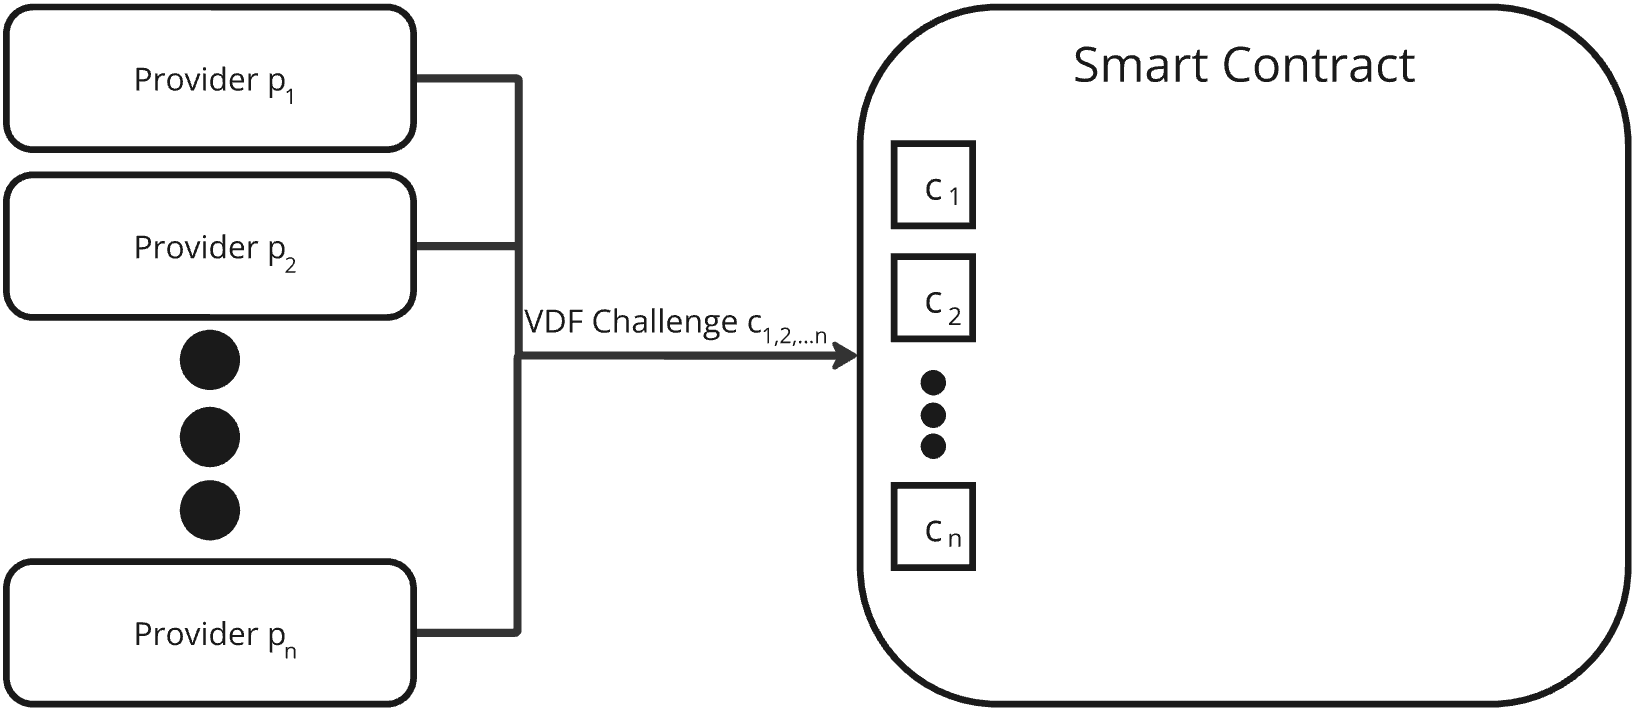
\includegraphics[width=0.8\textwidth]{images/protocol_commitment_phase.png}
    \caption{VDF Commitment Phase: Providers submit VDF commitments to the contract}
    \label{fig:protocol_commitment}
    \end{figure}
    
    \textit{Note}: Once all commitments are posted, the final output entropy value is deterministically locked but requires time $\tau$ to calculate, where:
    \begin{equation}
        \tau = \frac{T}{s}
    \end{equation}
    Here, $T$ is the number of sequential squaring operations from Pietrzak's VDF construction, and $s$ represents the number of modulo squaring operations per second achievable by the fastest available synchronous hardware \cite{9301680}. For security, we implement a timeout where the protocol aborts if any provider fails to commit within time $\tau$, resulting in penalties for non-compliant providers.
    
    \item \textbf{VDF Proof and Verification Phase}: To expedite the final output calculation, providers submit VDF checkpoints that can be verified in parallel by the contract. This process differs based on provider behavior:
    
    \begin{itemize}
        \item \textbf{Honest Case}: As illustrated in Figure~\ref{fig:verify_honest}, honest providers submit valid VDF proofs that are efficiently verified.
        
        \begin{figure}[H]
        \centering
        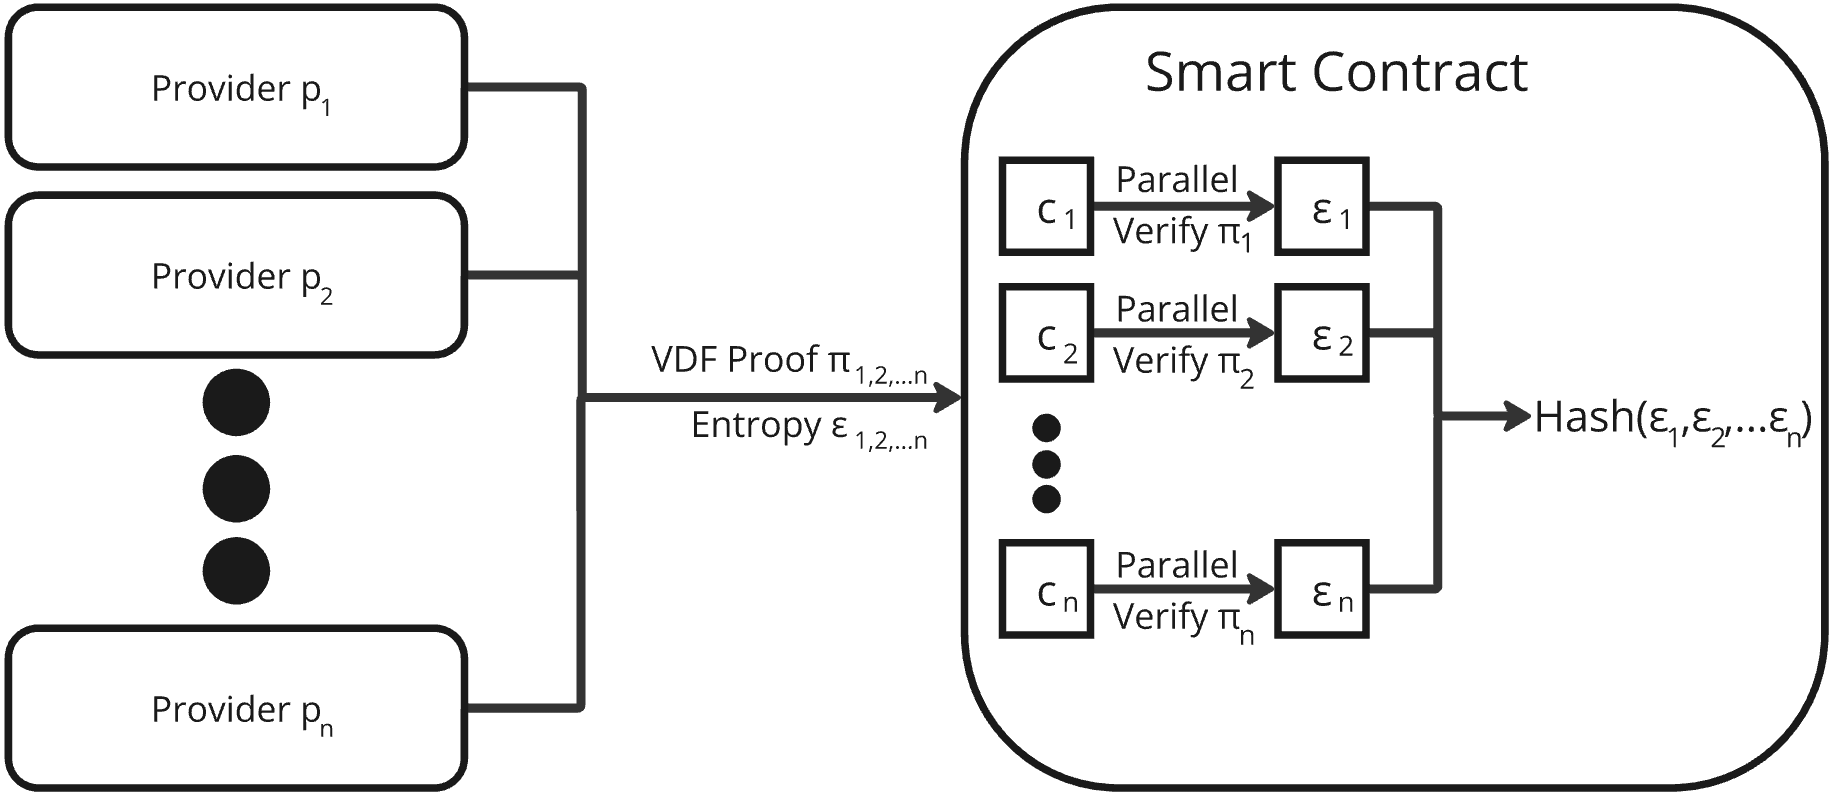
\includegraphics[width=0.8\textwidth]{images/verify-honest-case.png}
        \caption{Verification of Honest Provider: Valid VDF proofs are efficiently verified}
        \label{fig:verify_honest}
        \end{figure}
        
        \item \textbf{Malicious Case}: Figure~\ref{fig:verify_malicious} demonstrates how the protocol handles malicious providers through verification and penalties.
        
        \begin{figure}[H]
        \centering
        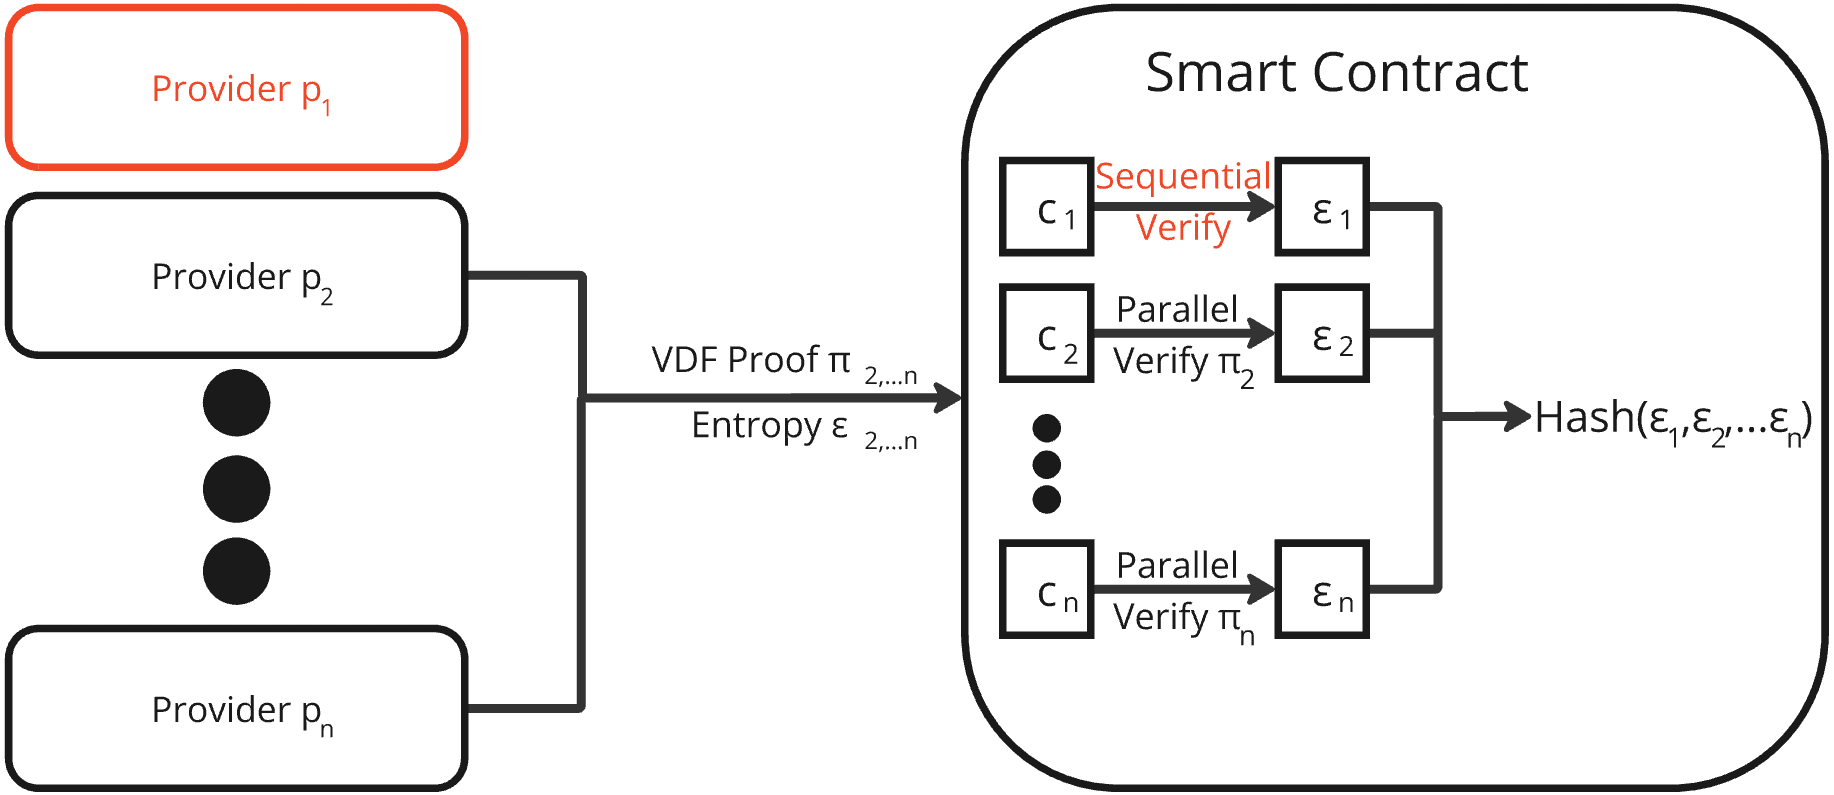
\includegraphics[width=0.8\textwidth]{images/verify-malicious-case.png}
        \caption{Malicious Providers during the proof stage are unable to abort the protocol, as their entropy value can be calculated sequentially from their VDF Challenge}
        \label{fig:verify_malicious}
        \end{figure}
    \end{itemize}
    
    \item \textbf{Entropy Aggregation}: After verification, all valid entropy values are aggregated using a cryptographic hash function to produce the final output entropy. This value remains unpredictable to any individual provider or participant, provided at least one provider acted honestly within the protocol.
\end{enumerate}
This design addresses the denial of service vulnerability discussed in Section~\ref{sec:commit_reveal_vulnerability}. Since all providers must submit VDF commitments and the final entropy value becomes deterministically locked once all commitments are provided, a malicious attacker can, at worst, only delay the outcome by the predetermined time $\tau$. This effectively solves the vulnerability where attackers could repeatedly force protocol restarts until achieving their desired outcome.

\subsection{Timing}
The timing characteristics of the RandAO protocol, using Pietrzak's VDF construction (see Section~\ref{sec:pietrzak}), are primarily determined by three key parameters:
\begin{itemize}
    \item $T$: The number of sequential squaring operations
    \item $\tau = T/s$: The actual time delay, derived from $T$ and the fastest available hardware's squaring speed $s$ \cite{9301680}
    \item $n$: The number of checkpoints that enables parallel verification
\end{itemize}

These parameters establish the protocol's timing bounds, with $T$ and the resulting $\tau$ determining the maximum delay an attacker can impose, and $n$ optimizing the verification speed through parallelization. Below we examine how these parameters influence the protocol's timing in both standard operation and failure cases.

\subsubsection{Case: Standard}
The RandAO protocol's timeline in the standard case can be broken down into four distinct phases, as illustrated in Figure~\ref{fig:timeline_usual}:

\begin{figure}[H]
\centering
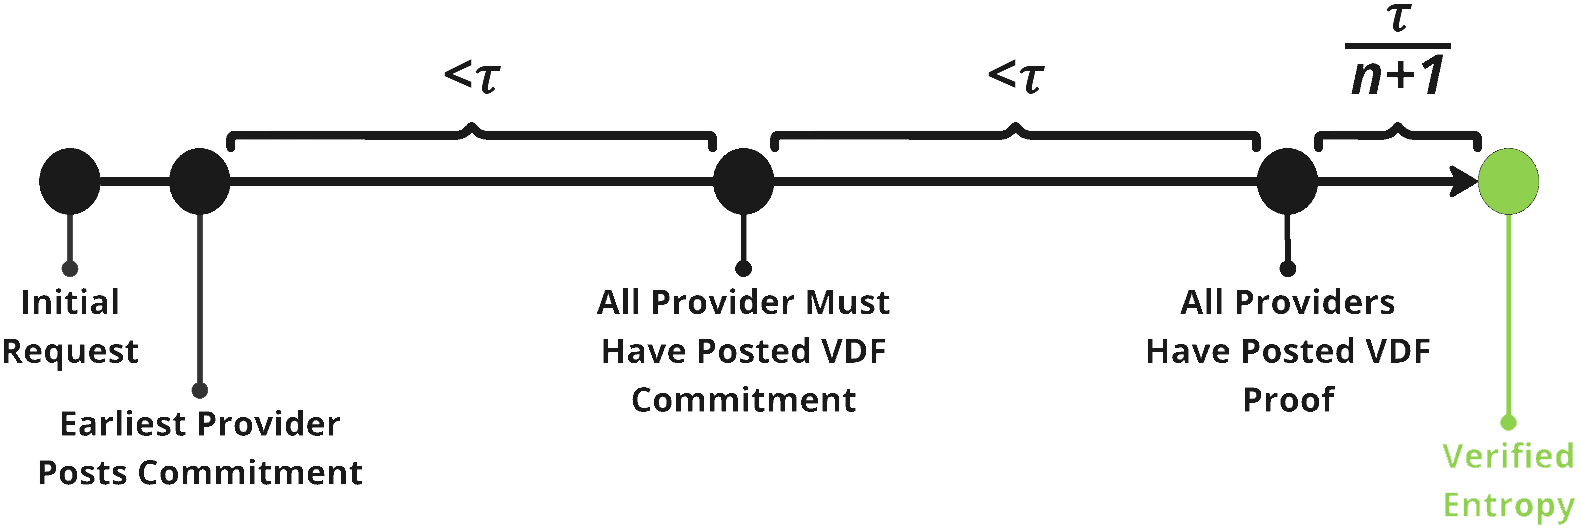
\includegraphics[width=0.8\textwidth]{images/timeline-usual-case.png}
\caption{Timeline of the standard case scenario showing the four main phases of the protocol execution}
\label{fig:timeline_usual}
\end{figure}

\begin{enumerate}
    \item \textbf{Initial Response}: The time between the initial random request and the first provider posting a VDF commitment. For competitive providers, this is expected to be near-instantaneous.
    
    \item \textbf{Commitment Window}: The period between the first and final provider's VDF commitment posts. This window must complete within time $\tau$ to prevent providers from gaining additional information. The protocol will abort if this exceeds time $\tau$. In practice, with competitive provider sets, this phase is expected to complete near-instantaneously.
    
    \item \textbf{Proof Submission}: The duration between the final provider's VDF commitment and all providers submitting their VDF proofs. With competitive provider sets, this phase is also expected to complete near-instantaneously.
    
    \item \textbf{Verification}: The time between all proofs being posted and the final verified entropy value being produced. Each proof segment takes time $\tau/(n+1)$ to verify, with all proofs and proof segments being verified in parallel:
    \begin{equation}
        t_{verify} = \frac{\tau}{n+1}
    \end{equation}
\end{enumerate}

\subsubsection{Case: Provider Fails to Post Proof}
When a provider fails to post their VDF proof, the protocol timeline changes as illustrated in Figure~\ref{fig:timeline_worst}:

\begin{figure}[H]
\centering
\includegraphics[width=0.8\textwidth]{images/timeline-worst-case.png}
\caption{Timeline showing the protocol phases when a provider fails to post their proof}
\label{fig:timeline_worst}
\end{figure}

The first two phases remain identical to the standard case:

\begin{enumerate}
    \item \textbf{Initial Response}: Near-instantaneous for competitive providers
    \item \textbf{Commitment Window}: Must complete within time $\tau$
\end{enumerate}

However, the final phase differs significantly:

\begin{enumerate}
    \item[3.] \textbf{Sequential Calculation}: The time required to sequentially calculate the non-compliant provider's entropy from their commitment, determined by $\tau$. This represents the worst-case scenario where the protocol must complete the VDF computation without the provider's proof.
\end{enumerate}

\subsection{Economic Security}\label{sec:economic_security}
RandAO's economic security model scales arbitrarily with the total staked collateral provided by the active provider set. A key strength of the protocol lies in its any-honest security guarantee: for any successful attack or collusion attempt to succeed, it must encompass every single member of the provider set. This creates a remarkably robust security model where a single honest citizen can uphold the integrity of an entire population - demonstrating that one individual's commitment to truth can outweigh any scale of corruption.

The security of the RandAO protocol scales with the relationship:

\begin{equation}
\mathcal{C} > \mathcal{R}
\end{equation}

where $\mathcal{C}$ represents the total collateral at risk for a given provider set. As long as the potential rewards $\mathcal{R}$ remain below this threshold, the economic security of the protocol remains intact, as successful manipulation would require complete collusion of all providers - a requirement that scales in difficulty as the provider set grows. Theoretically this protocol can remain secure against collusion for arbitrarily large rewards like universal lotteries, given a sufficiently collateralized provider set.
